\newpage
\section*{1-5}
Homeomorfizm pomiędzy
\begin{itemize}
  \item[1)] Sferą $S^n$
  \item[5)] $S^p \times S^q$ z utożsamionym do punktu zbiorem $\alpha \times S^q \cup S^p \times \beta$, dla $p + q = n$ gdzie $\alpha$ oraz $\beta$ są odpowiednio pewnymi wektorami z $S^p$ oraz $S^q$.
\end{itemize}
Z samego rachunku na zbiorach i z zadania 1-3 (sfera $S^n$ bez punktu homeomorficzna z $R^n$) otrzymujemy
$$
S^p \times S^q / \sim = (S^p \times (R^q \cup \{1\})) / \sim = (S^p \times R^q \cup S^p \times \{1\}) / \sim = ((R^p \cup \{1\}) \times R^q \cup S^p \times \{1\}) / \sim =  (R^p \cup \times R^q \cup \{1\} \times R^q \cup S^p \times \{1\}) / \sim
$$
ale
$$
\{1\} \times R^q \subset \{1\} \times S^q
$$
więc
$$
(R^p \cup \times R^q \cup \{1\} \times R^q \cup S^p \times \{1\}) / \sim = R^p \times R^q \cup \{c\} = R^n \cup \{c\}
$$
Po usunięciu $\{c\}$ (punktu, do którego utożsamiliśmy $S^p \times \{1\} \cup \{1\} \times S^q$) dostajemy homeomorfizm między $ S^p \times S^q / \sim \backslash \{c\}$  a $ R^n $.
Ale po dodaniu tego punktu $S^p \times S^q / \sim $ jest zwarte, więc homeomorficzne z jednopunktowym uzwarceniem $R^n$ - a to, z punktu 1.3 jest homeomorficzne z $S^n$.
\\

Wizualizacja dla $p = q = 2$

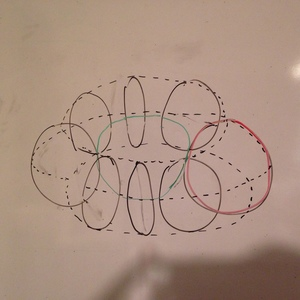
\includegraphics{a.jpg}\\
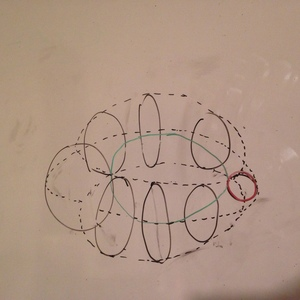
\includegraphics{b.jpg}\\
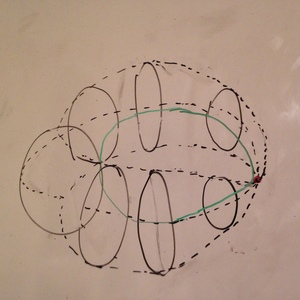
\includegraphics{c.jpg}\\
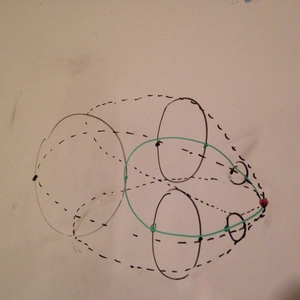
\includegraphics{d.jpg}\\
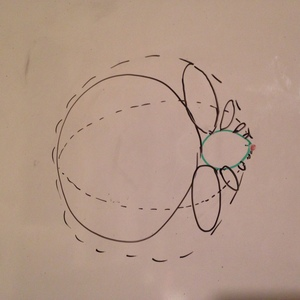
\includegraphics{e.jpg}\\
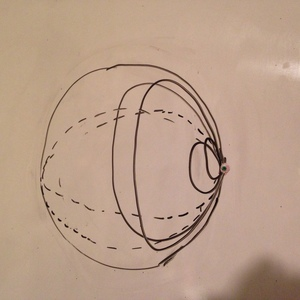
\includegraphics{f.jpg}\\